\documentclass[a4paper, 11pt]{article} %option para: draft mode not insert figure, give a faster preview
\usepackage[UTF8]{ctex} %for chinese
\usepackage{amsmath}    %for math
\usepackage{geometry}   %for page setting
\usepackage{graphicx}   % for insert graph
\usepackage{color}    %for link and code color
\usepackage{float}    %for graph table in the follow word
\usepackage[colorlinks,linkcolor=blue,anchorcolor=blue,citecolor=green]{hyperref} %for a linked ref

\setlength{\parindent}{2em} % maybe not use delete it ?
\geometry{left=3.0cm, right=3.0cm, top=3.0cm, bottom=3.0cm}

\graphicspath{{figure/}}


%%%%%%%%%%%%%%%%%%%%%%%%%%%%%%%%%%%%%%%%%%%%%%%%%%%%%%%%%%%%%%%%%%%%%%%%%%%%%%%%%%%%%%%%%%%%%%
%%%%             optional package default in comment to improve compile speed            %%%%

% \usepackage{physics}    %for a readable formulation


\usepackage[all]{hypcap} % use to jump to the top of figure/table rather than merely caption

\usepackage{fancyhdr}
\pagestyle{fancy} % leftmark is a build-in marco means the current higher level in markboth, right is a lower one

\addtolength{\headheight}{\baselineskip} % use to delete headheight waring
\fancyfoot[C]{\thepage}
\fancyhead[L]{\leftmark}
\fancyhead[R]{}
\renewcommand{\headrulewidth}{0pt}
\pagestyle{fancy}

% \usepackage[final]{listings} %for code use final to exclude draft mode to show whenever it is
% \definecolor{dkgreen}{rgb}{0,0.6,0}
% \definecolor{gray}{rgb}{0.5,0.5,0.5}
% \definecolor{mauve}{rgb}{0.58,0,0.82}

% \lstset{frame=tb,
%   language=c++,
%   aboveskip=3mm,
%   belowskip=3mm,
%   showstringspaces=false,
%   columns=flexible,
%   basicstyle={\small\ttfamily},
%   numbers=left, %none, right
%   numberstyle=\tiny\color{gray},
%   keywordstyle=\color{blue},
%   commentstyle=\color{dkgreen},
%   stringstyle=\color{mauve},
%   breaklines=true,
%   breakatwhitespace=true,
%   tabsize=2,
%   captionpos=b
% }
% \renewcommand{\lstlistingname}{源代码} % to change the prefix as 源码 not Listing
% \renewcommand{\lstlistlistingname}{源代码} % header name in list of listing
% % \usepackage{fontspec}
% % \setmonofont{Consolas} % set consolas in coding box, ONLY XeLaTeX so default comment remember a fontspec only used at the following


% \usepackage{wrapfig}  % for picutre on the paragraph right, cannot work with chinese par in pdflatex


% % \usepackage{fontspec} % for other font family


\usepackage{multirow} %for group row in a table


% Threeparttable
\usepackage{threeparttable}
\usepackage{booktabs}


% % drawing script tikz and Circuitlib 
% \usepackage{tikz}
% \usetikzlibrary{circuits.ee.IEC}
% \usetikzlibrary{positioning}

% \usepackage[american]{circuitikz}

%%%%%%%%%%%%%%%%%%%%%%%%%%%%%%%%%%%%%%%%%%%%%%%%%%%%%%%%%%%%%%%%%%%%%%%%%%%%%%%%%%%%%%%
%%%%%                         new recommand setting area                           %%%%

% % Count those in subsection
% \makeatletter
% \@addtoreset{equation}{subsection}
% \@addtoreset{figure}{subsection}
% \@addtoreset{table}{subsection}
% \makeatother
% \renewcommand {\thefigure} {\thesubsection{}.\arabic{figure}}
% \renewcommand {\thetable} {\thesubsection{}.\arabic{table}}
% \renewcommand {\theequation} {\thesubsection{}.\arabic{equation}}


% \newcommand{\parallelsum}{\mathbin{\!/\mkern-5mu/\!}} % parallesum for resistor
% \newcommand{\upcite}[1]{\textsuperscript{\textsuperscript{\cite{#1}}}}

%%%%%%%%%%%%%%%%%%%%%%%%%%%%%%%%%%%%%%%%%%%%%%%%%%%%%%%%%%%%%%%%%%%%%%%%%%%%%%%%%%%%%%%
%%%%%                         introduction section area                           %%%%


\title{\huge{\textbf{电子技术设计} \\ \textbf{环境舒适度综合测量仪}\\ \textbf{预习报告}}}
\author{
    \\
    \\
    \\
    \\
    \\
    \\
    \begin{tabular}{lll}
        班级: & 自72&自72\\
        姓名:& 高子靖&吴文绪\\
        学号: &2017010917&2017010910\\
    \end{tabular}
}
\date{}

\begin{document}


\maketitle
\thispagestyle{empty}
\setcounter{page}{0}
\newpage
\thispagestyle{empty}
\setcounter{page}{0}
\tableofcontents
\newpage
\section{选题背景及课题简介}
\subsection{选题背景}

随着我国经济不断发展,人民生活水平不断提高,人们对于室内生活环境的要求越来越高。另一方面,受到学科交叉的影响,以往的室内设计流程从较为主观的审美经验导向型,转向参考光学、心理学、生物学等学科知识的综合性设计。而迈向这样的设计,不免要进行一定的实验,标定室内环境参数是如何影响被试者对环境的评价的。

在传统的实验中\cite{2018slrxh},主要的流程是设置合适的室内环境,保证被试者进入实验后的几个小时待测参量基本不变(如使用空调控制室内温度,用灯光配合壁纸控制室内光强),当实验结束后,需要被试者根据这段时间的体验(如被试在环境中自习的专注度),回忆并填写相关问卷。可以看到,整套实验中,设置参数稳定的环境需要大量的前期准备,并且结束后的问卷统计环节有一定的主观性且效率较低。这些流程,均存在使用电子系统进行自动化的空间。

另外一方面,人们对于环境质量的要求体现在对PM2.5(当量直径等于或小于2.5微米的颗粒物体又被称为细颗粒、细粒、可入肺颗粒物)等指标的关注上。以PM2.5为例,它易悬浮在空气中,当被人体吸入肺部后易进入肺泡且沉积时间长,会对人的眼睛、鼻腔、上呼吸道等造成直接的伤害,也可能可导致心脏病或心血管疾病。正是这些健康敏感问题直接催生了PM2.5检测仪和其他家用空气质量测量仪等电子产品的出现。广阔的市场为我们提供了丰富的已有设计方案作为对比参考,能让我们在前人的基础上综合优点、补足缺陷,继续进步,完成对环境参数的集成测量。

此外,作为一个应用于室内环境试验的测量仪,我们还将被试者评价环境这一环节整合了进来。在这个系统中,我们面向的是专注度环境测试,被试者常接到的任务是在待测环境中自习,评价自己的自习专注度。我们注意到,自习时的不专注可以抽象为人的上半身离开桌面的正上方,这样的现象的检测可以通过红外传感器或微波雷达这样的生物检测模块实现。使用了这样的方法后,一方面我们将主观的问卷评价进行了指标化和客观化,另一方面,电子系统采集统计数据免去了统计问卷的过程,让整个实验更为自动化。在与实际环境问题结合也是我们与“智能检测”主题相关的出发点。


\subsection{课题简介}
\par{} 我们以PM2.5检测仪作为出发点,进而加入对空气湿度,温度,气压及其他有害气体的检测等作为指标,集成为一款环境舒适度综合测量仪,并通过蓝牙模块与手机进行连接,能够传输一份格式化的环境检测报告到用户的手机中去,以及LCD进行显示。
\subsubsection{测量指标}
\par{} 本课题围绕“智能检测”的主题,拟在设计中加入对以下指标的检测:
\begin{itemize}
    \item 大气PM2.5颗粒浓度
    \item 空气湿度,也即湿蒸汽中液态水分的质量占蒸汽总质量的百分比
    \item 环境温度,温度对人体对环境舒适度的感知造成直接的影响
    \item 大气压强,环境的气压会对人体生理以及心理产生影响
\end{itemize}
\par{} 以上我们初步计划进行测量的指标,并对相应的测量数据进行存储与发送。通过以上的四个指标能够初步反映所处环境的基本状况,包含健康指标和舒适指标,提供给用户后用户可根据相应的测量结果对湿度,温度等进行调节或做好大气污染的相应防护措施,从而提高环境的舒适度。


\subsubsection{实现方法}
\par{} 我们在简介部分只给出实现方案的基本框图,具体的实现方案细节将于第\ref{sect1}部分中给出。那么电路框图如下图[\ref{img1}]所示:
\begin{figure}[H]
    \centering
    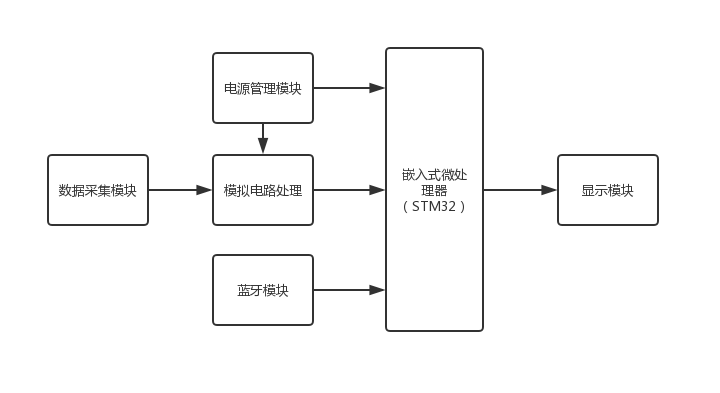
\includegraphics[scale = 0.58 ]{1-1.png}
    \caption{设计总体框图}
    \label{img1} 
  \end{figure}
\par{} 由上图可知,我们通过传感器进行数据采集,进一步进行模拟电路对数据处理,再通过模数转换电路驱动单片机,除此之外由电源管理模块为单片机以及模拟部分提供稳压电源,并另行有蓝牙模块与手机进行通讯,而数字部分的处理全部交由STM32完成,最终进行显示。

\subsubsection{结果反馈方法}
\par{} 我们计划使用LED或LCD显示屏将收集到的数据进行显示,显示内容包括以上叙述的测量指标,时间日期等,并加入阈值报警,若超过规定的阈值,则通过蜂鸣器进行报警。其次利用蓝牙模块与手机进行连接,将测量结果可以在用户手机上进行实时的显示,能够极其方便的获取当前环境情况。

\section{方案比较与选择}\label{sect1}
\par{} 通过我们对文献的查阅以及阅读,可以看到大多数基于单片机的大气环境检测系统,都是选择一款合适的单片机或其他微处理器作为主控,也即系统的核心,通过各个传感器与主控的连接进行数据的处理,最后通过LCD显示屏来进行结果的反馈。在整体上这些方案大同小异,但为我们的设计提供了思路与基础,而方案的选择也体现在细节方面的主控芯片的选择以及传感器的选择。
\subsection{文献方案叙述}
\par{} 首先叙述总结在文献中获得的方案设计,为了比较不同,我选择了其中的一篇基于ARM的多功能环境检测系统与基于STC90C51单片机的多功能检测系统分别进行介绍。
\subsubsection{基于ARM的多功能环境检测系统}
\par{} 首先我查阅到ARM处理器是英国Acorn有限公司设计的低功耗成本的第一款RISC微处理器。具有体积小、低功耗、低成本、高性能等优势。而在文章\footnote{引用文章,见于参考文献1中}的设计中以ARM作为主控单元,还包括PM2.5传感器单元、温湿度传感器单元、液晶显示屏单元、语音实时播报单元、外部事件触发单元\cite{qal2017jy}。整体可以由如下的框图实现:
\begin{figure}[H]
  \centering
  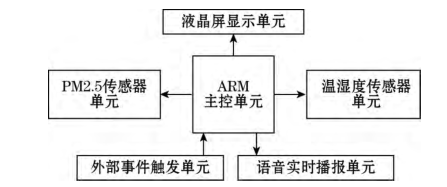
\includegraphics[scale = 0.7 ]{1-2.png}
  \caption{ARM设计总体框图}
  \label{img2} 
\end{figure}
\par{} 主控单元与模块化的思路是对于类似系统设计的基本思路,也是我们阅读的文献的共同思路,而其他传感单元由于可替换性因此需要我们加以选择。
\par{} 首先主控单元采用了ARM,可使用KEIL4编译软件环境进行开发,同时可利用C语言进行程序的编写,开发时十分方便快捷。
\par{} PM2.5浓度传感器其采用PMS70XX系列超薄数字式通用颗粒物浓度传感器。经查阅其中文手册,得知该传感器工作原理图如下所示:
\begin{figure}[H]
  \centering
  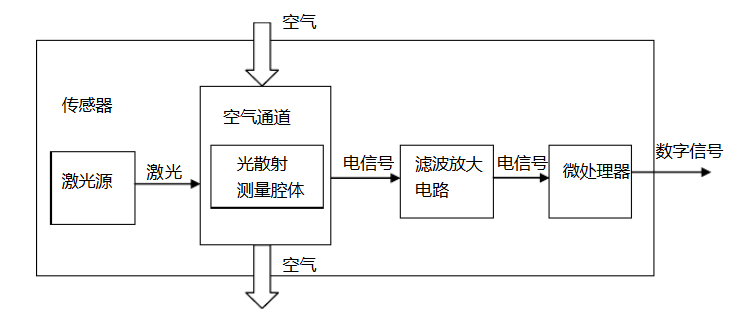
\includegraphics[scale = 0.65 ]{1-3.png}
  \caption{PM570XX系列传感器}
  \label{img3} 
\end{figure}
\par{} 其主要通过激光源发射激光经过腔体,在腔体内由于颗粒物浓度不同导致散射光强不同,进而能够转化为电信号,从而利用反射光强来反馈出细微颗粒物的浓度,直流供电电压为5V,最大工作电流为100mA,工作温度范围为$-20^{\circ} C\sim 50^{\circ}C$,传输协议为默认波特率9600Kbps,无校验位,有一位停止位。
\par{} 液晶显示屏采用一个3.5英寸的TFT LCD液晶屏,320$\times 240$像素,26万色,支持触摸屏功能,能够较好的进行显示。其他单元模块芯片不再赘述。
\subsubsection{基于STC90C51的检测系统}
\par{} 该检测系统为我所阅读文献中另一篇较具有代表性的文献,其设计除主控单元不同外,在传感器的选取上也与上一个单元有所不同,因此特此拿来与上一个系统进行比较分析,同样首先从整体框图上说明该系统的工作原理。
\begin{figure}[H]
  \centering
  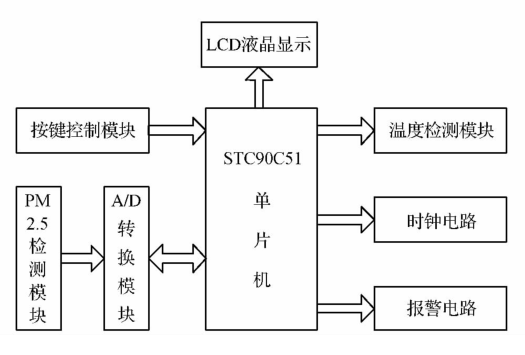
\includegraphics[scale = 0.65 ]{1-4.png}
  \caption{STC90C51总体框图}
  \label{img4} 
\end{figure}

\par{} 可见该系统总体框图与ARM系统基本相似,均以单片机作为主控单元,各模块电路通过硬件连接与主控单元进行相连与交互,只是该系统的设计中外接部分单元电路的功能不同。
\par{} 其主控单元为STC90C51单片机,为一款高速低功耗单片机,其在编译环境以及编程的方便性与可移植性等方面与其他单片机并无较大差别,因此也非选择的重点。
\par{} 其PM2.5检测模块使用的传感器为GP2Y1050AU0F灰尘传感器,是夏普公司开发的二代PM2. 5传感器\cite{cz2016yz},输出电压在$0\sim 3.5V$的范围内,电流损耗最大为20mA。在无尘时输出电压为0V,其原理如下图[\ref{img5}]所示:
\begin{figure}[H]
  \centering
  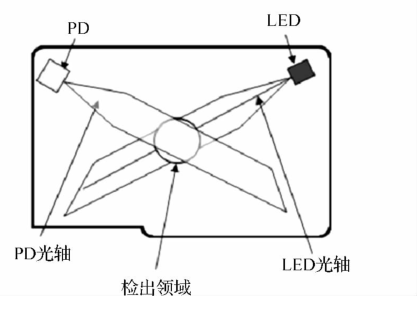
\includegraphics[scale = 0.65 ]{1-5.png}
  \caption{GP2Y1050AU0F灰尘传感器结构}
  \label{img5} 
\end{figure}
\par{} 检测原理为灰尘或烟雾颗粒通过防尘通气孔进入装置,红外发光二极管发射红外线到颗粒物上,光敏三极管接收其散射光信号。可见其原理与PM570XX系列相似,第二代PM2. 5传感器能随使用时间的增长自动计算和优化损耗\cite{wl2016dgn},能够在较长时间的使用后保证输出数据的准确性,相对而言体现了此传感器的优势。
\par{} 在此设计中采用ADS7822进行模数转换,其输入与传感器的模拟输出相连,作用是将传感器输出的模拟电压信号经过 A/D 转换,再由单片机数据采集、计算、处理。ADS7822是TI公司的低功耗,高性能12位A/D转换芯片,正常模式下典型功耗为0.54mW。
\par{} 其使用的温度模块采用了DS18B20数字温度传感器,其具9 Bit至12Bit的摄氏温度测量精度,测量范围为-55$\sim +125^{\circ}C$,可以直接由数据线进行供电而不需要外部电源,因此可以外部电源的使用。
\par{} 综上所述介绍的两种具有多功能的PM2.5检测仪,为我们的设计提供了基本的思路与选择的方向,我们旨在设计出具有更多功能的环境舒适度测量仪,以上pm2.5的多功能模块的总体方案为我们的设计的重要部分,接下来我将继续介绍我们的整体方案选择。
\subsection{方案选择}
\par{} 综合考虑我们选用Arduino单片机作为主控模块,其余相应单元模块进行了芯片的初步选择,这既考虑到芯片供电电压的选取与我们电源管理电路模块尽量相符,又兼并考虑了芯片的精度,工作范围等条件,下面依次介绍我们所选取的芯片,电路框图类比于以上两种设计,我们的设计如下:
\begin{figure}[H]
  \centering
  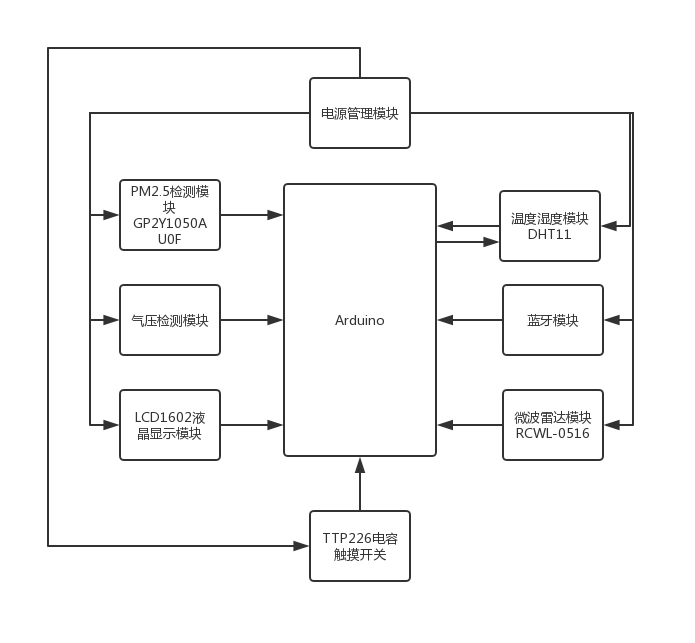
\includegraphics[scale = 0.45 ]{1-n.png}
  \caption{简略框图}
  \label{img6} 
\end{figure}
\subsubsection{单片机Arduino}
\par{} Arduino就是主要以以AVR单片机为核心控制器的单片机应用开发板,其开发人员开发了简单的函数,还有许多应用库,这样就不用直接去操作寄存器。Arduino相对于传统的单片机而言,可以不用去了解去硬件的知识去进行开发,并且利用C语言进行开发,指令的可读性更强,Arduino还有很多第三方库,包含了写好的函数,每个函数有各自的功能,可供调用。常用的库有标准链接库,通信库,传感器库,音效和声波库,电机和脉宽调制库,计时器库,实用工具库等。因此我们选择Arduino作为主控模块。


\subsubsection{GP2Y1050AU0F灰尘传感器}
\par{} 我们使用该传感器作为PM2.5检测模块的核心部分,GP2Y1050AU0F灰尘传感器为夏普公司的二代PM2.5传感器,主要功能为烟灰或室内灰尘等空气中的粉尘处于检测范围内时,由于这些粉尘而散射的光射入光接收元件作为电压输出。传感器的一般性能如下表[\ref{tab1}]所示:
\begin{table}[H]
  \centering
  \caption{绝对最大额度}
  \label{tab1}
  \begin{threeparttable}
    \small
    \begin{tabular} {p{80pt}p{80pt}p{80pt}p{80pt}}
      \hline
      项目&记号&额定&单位\\
      \hline
      动作电压&Vcc&$4.8\sim 5.2$&V\\
      动作温度&Topr&$-10\sim +65$&$^{\circ}C$\\
      保存温度&Tstg&$-20 \sim +80$&$^{\circ}C$\\
      \hline
    \end{tabular}
    \small
  \end{threeparttable}
\end{table} 
\par{}其电气的光学特性如下表[\ref{tab2}]所示:

\begin{table}[H]
  \centering
  \caption{电气的光学特性}
  \label{tab2}
  \begin{threeparttable}
    \small
    \begin{tabular} {p{80pt}p{80pt}p{80pt}p{80pt}p{80pt}}
      \hline
      项目&记号&MIN&MAX&单位\\
      \hline
      检测感度&K&0.35&0.65&V/$(0.1mg/m^3)$\\
      电流&Icc&———&20&mA\\
      \hline
    \end{tabular}
    \small
  \end{threeparttable}
\end{table} 
\par{}其中的检测感度K为关于粉尘浓度$(0.1mg/m^3)$变化时的输出电压变化量所规定的。其输出方式有模拟端口和串口两种方式,其中模拟端口输出电压$V_o$乘以系数K得到灰尘浓度值,单位为$\mu g/m^3$,串口输出经通信转换后得到$V_o$值,传输特性如下所示:

\begin{figure}[H]
  \centering
  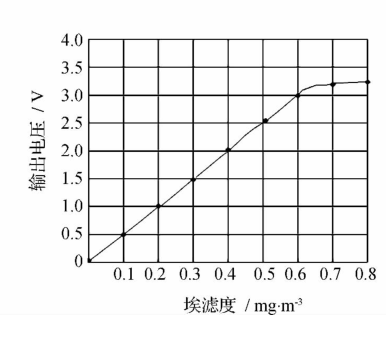
\includegraphics[scale = 0.65 ]{1-6.png}
  \caption{输出特性曲线}
  \label{img7} 
\end{figure}



\subsubsection{DHT-11温度湿度传感器}
\par{} DHT11数字温湿度传感器是一款含义已校准数字信号输出的温湿度复合传感器。其中的传感器包括一个电容式感湿元件和一个NTC测温元件,并和一个高性能8位单片机直接相连,可以应用于除湿器、农业、冷链仓库等方面,而这里我们使用其作为环境检测的温湿度模块,由于其数字信号输出的特性,能够方便的与单片机相连,并且将精确校准的信号交由单片机进行处理。因此我们选用DHT-11模块。传感器的外形尺寸如下图[\ref{img8}]所示
\begin{figure}[H]
  \centering
  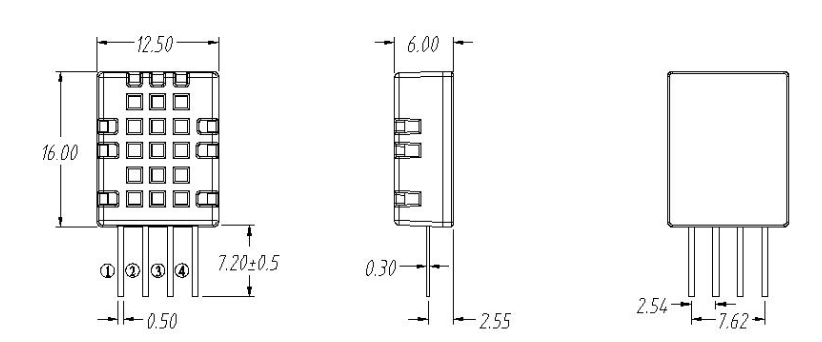
\includegraphics[scale = 0.58 ]{1-7.png}
  \caption{DHT11外形尺寸}
  \label{img8} 
\end{figure}

\par{}其中的引脚为:1.VDD供电为$3.3\sim 5V$DC,2.DATA串行数据,单总线3.NC空脚4.GND接地,电源负极。
\par{} 湿度的量程范围为$5\sim 95 \%RH$,温度的量程范围为$-20\sim 60^{\circ}C$。而在$25^{\circ}C$的条件下,相对湿度的精度为$\pm 5\%RH$,温度的精度为$\pm 2^{\circ}C$,电气特性如下表[\ref{tab3}]所示:
\begin{table}[H]
  \centering
  \caption{电气特性}
  \label{tab3}
  \begin{threeparttable}
    \small
    \begin{tabular} {p{70pt}p{70pt}p{70pt}p{70pt}p{70pt}p{70pt}}
      \hline
      参数&条件&MIN&type&max&单位\\
      \hline
      供电电压&&3.3&5.0&5.5&V\\
      供电电流&&0.06&&1.0&mA\\
      采用周期&测量&&>2&&S/次\\
      \hline
    \end{tabular}
    \small
  \end{threeparttable}
\end{table}

\subsubsection{LCD1602液晶显示屏}
\par{} LCD1602是一种工业字符型液晶,能够同时显示16x02即32个字符。LCD1602液晶显示的原理是利用液晶的物理特性,通过电压对其显示区域进行控制,即可以显示出图形。其引脚功能在此不再赘述,外形如下所示:

\begin{figure}[H]
  \centering
  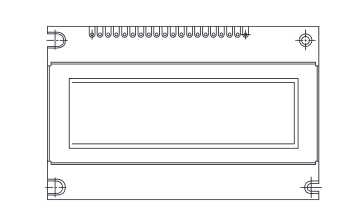
\includegraphics[scale = 0.58 ]{1-8.png}
  \caption{DHT11外形尺寸}
  \label{img9} 
\end{figure}

\par{} 该模块的电气特性如下表所示:
\begin{table}[H]
  \centering
  \caption{电气特性}
  \label{tab4}
  \begin{threeparttable}
    \small
    \begin{tabular} {p{70pt}p{70pt}p{70pt}p{70pt}p{70pt}p{70pt}}
      \hline
      参数&条件&MIN&type&max&单位\\
      \hline
      输入电压&VDD=+5V&4.5&5.0&5.5&V\\
      输入电流&VDD=5V&1.0&1.4&mA\\
      \hline
    \end{tabular}
    \small
  \end{threeparttable}
\end{table}

\subsubsection{TTP226电容触摸开关}
\par{}TTP226是一款接触板检测IC,提供8个接触键。低功耗和宽工作电压是接触键在DC或AC应用中的特点。其工作特性如下所示:
\par{}工作电压为2.0$\sim$5.5V,工作电流在VDD=3v时典型值80$\mu A$,最大值160$\mu A$,输出刷新率在VDD=3v时约55Hz。
\begin{figure}[H]
  \centering
  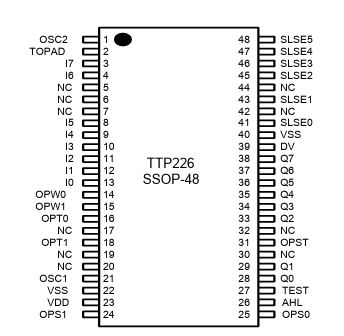
\includegraphics[scale = 0.58 ]{1-9.png}
  \caption{TTP226封装引脚图}
  \label{img10} 
\end{figure}
\par{} 其应用为取代传统的按键,由于我们使用的液晶显示屏一次性显示字符有限,因此在本设计中借助于此IC来进行不同检测指标的选择显示。

\subsubsection{RCWL-0516微波雷达}
\par{} RCWL-0516微波雷达采用多普勒雷达技术,是专门检测物体移动的微波感应的模块。具有灵敏度高,感应距离远,可靠性强、可以穿越障碍物进行检测的特点,这里我们基于设计出发时将环境舒适度以学生自习作为标准,因此会对环境内的人体姿态例如抖腿、玩手机等动作进行捕捉,希望借助此模块来探测人手是否静放于桌面上,或室内其他人是否有抖腿的行为,将由此模块进行捕捉。
\par{} 此模块外观如下所示:
\begin{figure}[H]
  \centering
  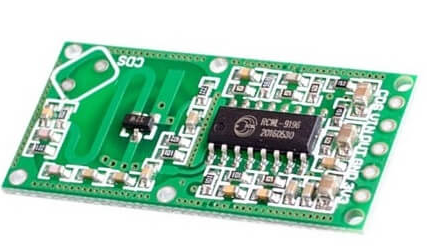
\includegraphics[scale = 0.6 ]{1-10.png}
  \caption{RCWL-0516外观图}
  \label{img10} 
\end{figure}
\par{} 其中部分引脚的名称与管脚定义的对应关系如下:
\begin{table}[H]
  \centering
  \caption{管脚对应关系}
  \label{tab5}
  \begin{threeparttable}
    \small
    \begin{tabular} {p{70pt}p{70pt}p{70pt}p{70pt}p{70pt}}
      \hline
      名称&MIN&type&max&单位\\
      \hline
      工作电压&4&&28&V\\
      工作电流&&2.8&3&mA\\
      探测距离&5&7&9&M\\
      输出电压&3.2&3.3&3.4&V\\
      \hline
    \end{tabular}
    \small
  \end{threeparttable}
\end{table}
\par{}部分性能参数如下:
\begin{table}[H]
  \centering
  \caption{性能参数}
  \label{tab6}
  \begin{threeparttable}
    \small
    \begin{tabular} {p{80pt}p{220pt}}
      \hline
      名称&管脚定义\\
      \hline
      3V3&3V3电源输出\\
      GND&地\\
      OUT&控制输出,检测到有移动物体输出高电平\\
      VIN&输入电压4-28V\\
      CDS&使能控制芯片,低于0.7V,OUT一直输出低电平\\
      \hline
    \end{tabular}
    \small
  \end{threeparttable}
\end{table}

\section{基于WEBENCH的电源电路仿真}

电路使用标称值为$9V$的锂电池作为电源。对于主控模块arduino其板载有稳压模块,对于$7-12V$范围内波动的电压,均能正常工作。故而电源管理电路主要给外围的各类传感器使用。查看前述各传感器模块的工作电压范围,电源管理电路仅做$5V$输出即可。将各模块的工作电流最大值进行求和得到的电流$I_\Sigma \approx 300mA$。考虑后续可能增加其他模块和安全工作余量的考虑,在设计电源时取$I_{o(max)} = 1.5A$。标称值为$9V$的锂电池,通过官方数据手册得到其输出电流波动范围大约为$8 \sim 10V$,以此作为$V_{in}$的范围,输入WEBENCH后,在所给仿真方案中挑选了基于TPSM84205EAB的电源管理电路方案。其生成的详细报告在附录\ref{sec:webench_report}中给出,这里主要摘取其关键的参数和补充的仿真进行分析。

此外,在WEBENCH生成的这个方案中,不支持波特图仿真和热仿真。故而从其他波形图验证设计合理性的流程中,我们应当保证一定的余量。具体而言是在稳态波形中,输出电压的波动应当足够小,从另一方面达成用波特图验证自激振荡不会发生的目的;在所有波形中,各极限指标应当与阈值有一定的差距,保证在环境温度变化时,电路各输出参数仍满足要求。

\subsection{软启动仿真}

\begin{figure}[H]
    \centering
    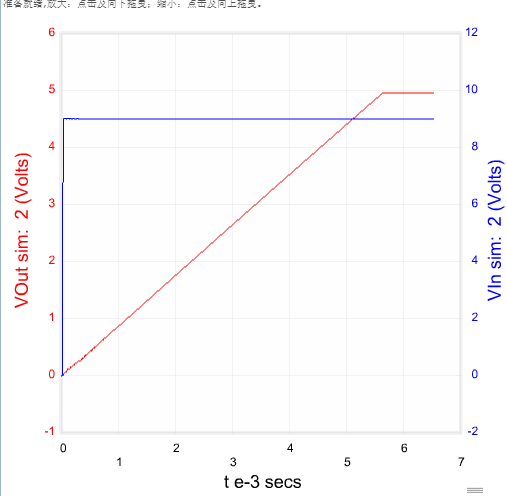
\includegraphics[width = 0.4\textwidth]{startup_sim.png}
    \caption{$V_{in}, V_{out}$软启动仿真波形}
\end{figure}

可以看到,为了消除自激振荡而在输入输出端的增加的两个电容,让$V_{out}$的变化减慢了,在开关合闸后,需要一定的时间给两电容充电,并且等到芯片内部的稳压管和放大模块建立合理的直流电压值后,$V_{out}$才在设定工作范围下工作。从图中具体读得在大约$5.5ms$后$V_{out}$稳定,电路开始正常工作。

从应用背景,我们可以推测整体系统在工作后不常断电,故虽减小电容容值可以减小合闸后的转换时间,但是会减小自激振荡的幅度裕度,在这两个参数指标的取舍上,结合实际应用背景和可得的电容,我们使用了原来的容值设置,$C_{in} = 10\mu F, C_{out} = 47\mu F$。

\subsection{稳态仿真}

\begin{figure}[H]
    \centering
    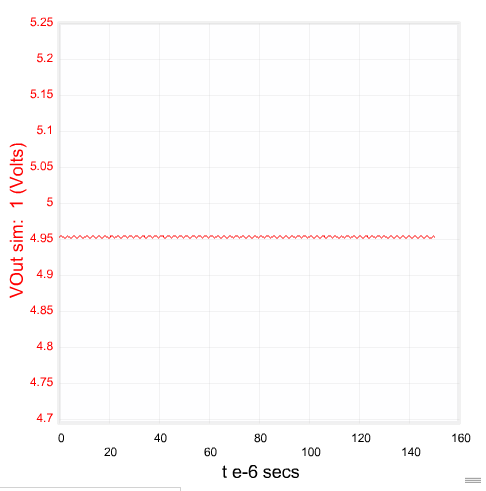
\includegraphics[width = 0.45\textwidth]{steady_state_sim.png}
    \caption{$V_{in}, V_{out}$稳态仿真波形}
\end{figure}

稳态仿真中,我们可以看到输出电压的纹波情况。由于使用的是线性稳压电路而非开关稳压电路,故在稳态时,没有其他工作状态随时间有明显变化的元件,仿真波形仅做排除稳压器自激振荡的可能性和电路工作状态合理稳定的验证。

\subsection{输入瞬态响应仿真}

\begin{figure}[H]
    \centering
    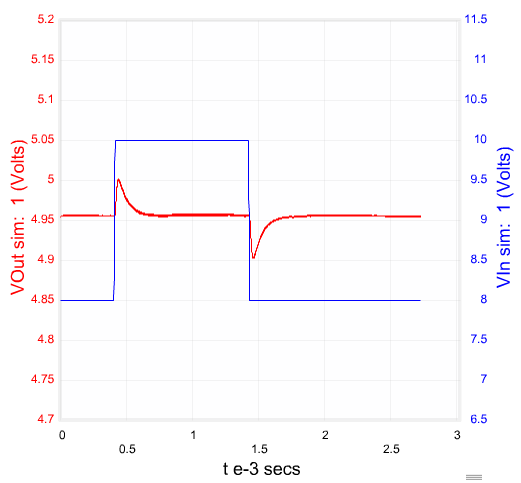
\includegraphics[width = 0.45\textwidth]{input_transient.png}
    \caption{$V_{in}, V_{out}$输入瞬态仿真波形}
\end{figure}

输入瞬态响应中,在保证稳态的情况下,$V_{in}$从最小值$8V$跳变到允许最大值$10V$再回跳。从波形中可以知道,在电压变化后且达到稳态时,$V_{out}$几乎不变,符合电源电路的一大要求——输出电压几乎不随输入电压的变化而变化。之后再观察转换暂态,可以看到输出变动量的峰值和谷值约为$0.05V$,变化较小,且在供电设备(即各传感器模块)的允许工作电压范围内,设计符合要求。

\subsection{负载瞬态响应仿真}

\begin{figure}[H]
    \centering
    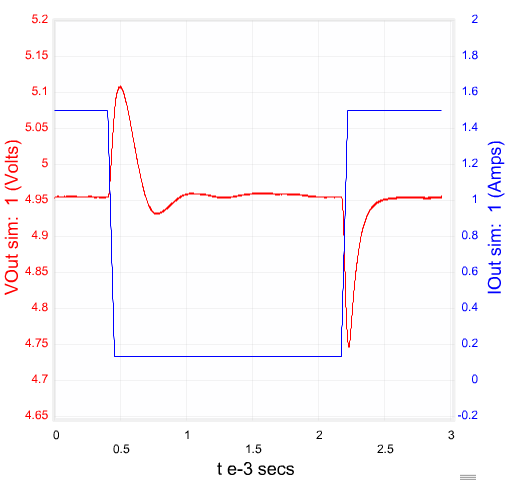
\includegraphics[width = 0.45\textwidth]{load_transient_sim.png}
    \caption{$V_{in}, V_{out}$负载瞬态仿真波形}
\end{figure}

负载瞬态响应中,在保证稳态的情况下,$I_L$从最大值$1.5A$跳变到允许最大值$0.15A$再回跳。从波形中可以知道,在电压变化后且达到稳态时,$V_{out}$几乎不变,符合电源电路的另一大要求——输出电压不随合理变化范围内的负载变动而变化。之后再观察转换暂态,可以看到输出变动量的峰值和谷值约为$0.2V$,相对于上一节中的输入瞬态响应,负载变化响应的变化较大,可能存在一定的危险。

在设备工作时,电路各传感器处于常开状态,不会产生明显的负载变化,在进行通信时,由于无线收发的存在,会产生较大的负载变动,导致输出电压的变化。电压变动大会比较明显影响模拟量传感器的测量精度,让变动时期测得的数据变得不可靠。可能考虑到这一点,我们在选取通信模块时,选用$3.3V$的低功耗模块,并作为arduino的负载而非电源管理电路的负载,合理规避了负载变化导致的较为明显的电源输出电压变化的可能性。

\subsection{电源效率和纹波电压}

\begin{figure}[H]
    \centering
    \begin{minipage}[H]{0.48\textwidth}
        \begin{figure}[H]
            \centering
            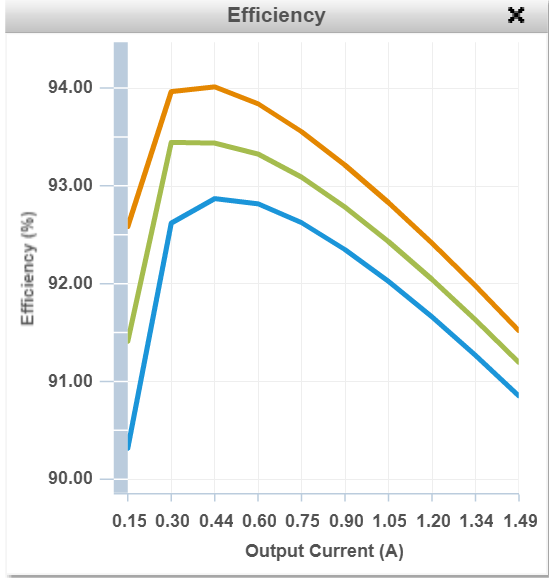
\includegraphics[width = 0.8\textwidth]{efficiency-I.png}
            \caption{$\eta \sim I_{out}$的变化关系}
        \end{figure}
    \end{minipage}
    \begin{minipage}[H]{0.48\textwidth}
        \begin{figure}[H]
            \centering
            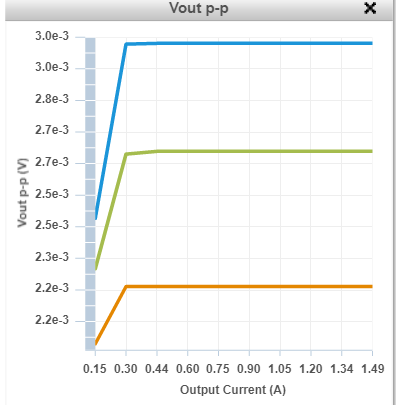
\includegraphics[width = 0.8\textwidth]{Vpp-I.png}
            \caption{$\Delta V \sim I_{out}$的变化关系}
        \end{figure}
    \end{minipage}
\end{figure}

上图中的橙色线为$V_{in} = 8.0V$,绿色线为$V_{in} = 9.0V$,蓝色线为$V_{in} = 10.0V$时的输出情况。可以看到在合理的工作电流变化范围内,$\eta > 90\%$且在目前设计的典型负载电流$I = 0.3A$的情况下,大约能得到最高的电源效率。纹波电压随$I_{out}$的变化较小,并且纹波电压本身的值较小,说明电源管理电路输出的电压在大范围内符合好的“直流电压”的要求。

\section{电路框图}
\par{} 此电路框图类比于第二部分的文献中框图,以Arduino为核心主控单元,其余各部分功能电路模拟输出或数字输出均接入Arduino中进行数据的处理与存储,其中各个部分单元用到的芯片的简介均在第二部分给出,因此各部分功能在此简要叙述:
\begin{itemize}
\item 电源管理模块输出5V电压为整个系统进行供电
\item PM2.5模块负责检测大气细微颗粒物
\item 气压检测模块检测大气压强是否在舒适范围内
\item TTP226电容触摸开关进行显示屏的显示内容选择与切换
\item 蓝牙模块负责与手机通信,将结果反馈至手机
\item 微波雷达模块负责监视室内人体姿态情况,是否满足“舒适”条件
\item LCD1602负责结果的直接显示,通过液晶显示屏获取测量结果


\end{itemize}
\par{} 而最终的框图相较于第一部分有所改进与补充,并修改STM32为Arduino,如下图[\ref{img6}]所示:



\begin{figure}[H]
  \centering
  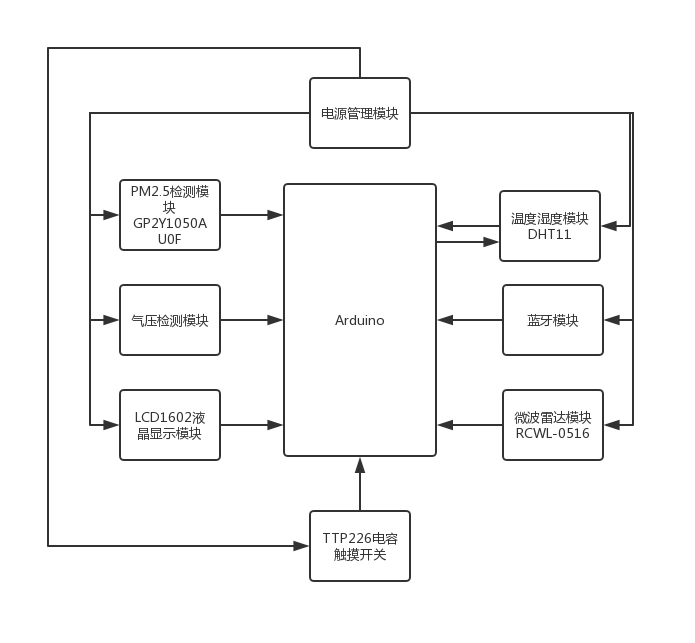
\includegraphics[scale = 0.45 ]{1-n.png}
  \caption{简略框图}
  \label{img6} 
\end{figure}



\section{数字系统流程图}

整体而言,数字系统主要实现以下几个功能:

\begin{itemize}
    \item 对于不同传感器的巡检管理。系统涉及的传感器较多、IO口较少且不需要同步检测,故而采用巡检这样的外围控制模式。
    \item 对于传感器和DA转换模块最后发来的数字量做一定的预处理或者说数字滤波。在不同的实验设置下,实验者关心的时间跨度,参量阈值不尽相同,这些参数的变化通过数字系统对前端信号预处理流程的不同得以实现。
    \item 对于键盘输入的响应管理,用于切换仪器的测量模式,显示不同的测量。
    \item 对于实验数据的同步,用于驱动通信模块,回传实验数据用以分析。
\end{itemize}

对于这几大功能,结合实际测量过程,得到数字系统的流程图如下:

\begin{figure}[H]
    \centering
    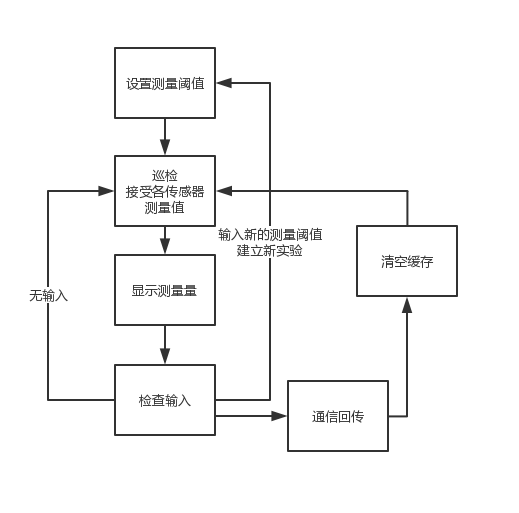
\includegraphics[width = 0.618\textwidth]{digital_flow.png}
    \caption{数字系统流程图}
\end{figure}


\newpage
\bibliographystyle{plain}
\addcontentsline{toc}{section}{参考文献}
\bibliography{yuxi.bib}

\newpage
\appendix
\pagestyle{empty}
\section{WEBENCH生成的仿真报告}
\label{sec:webench_report}

\begin{figure}[H]
    \centering
    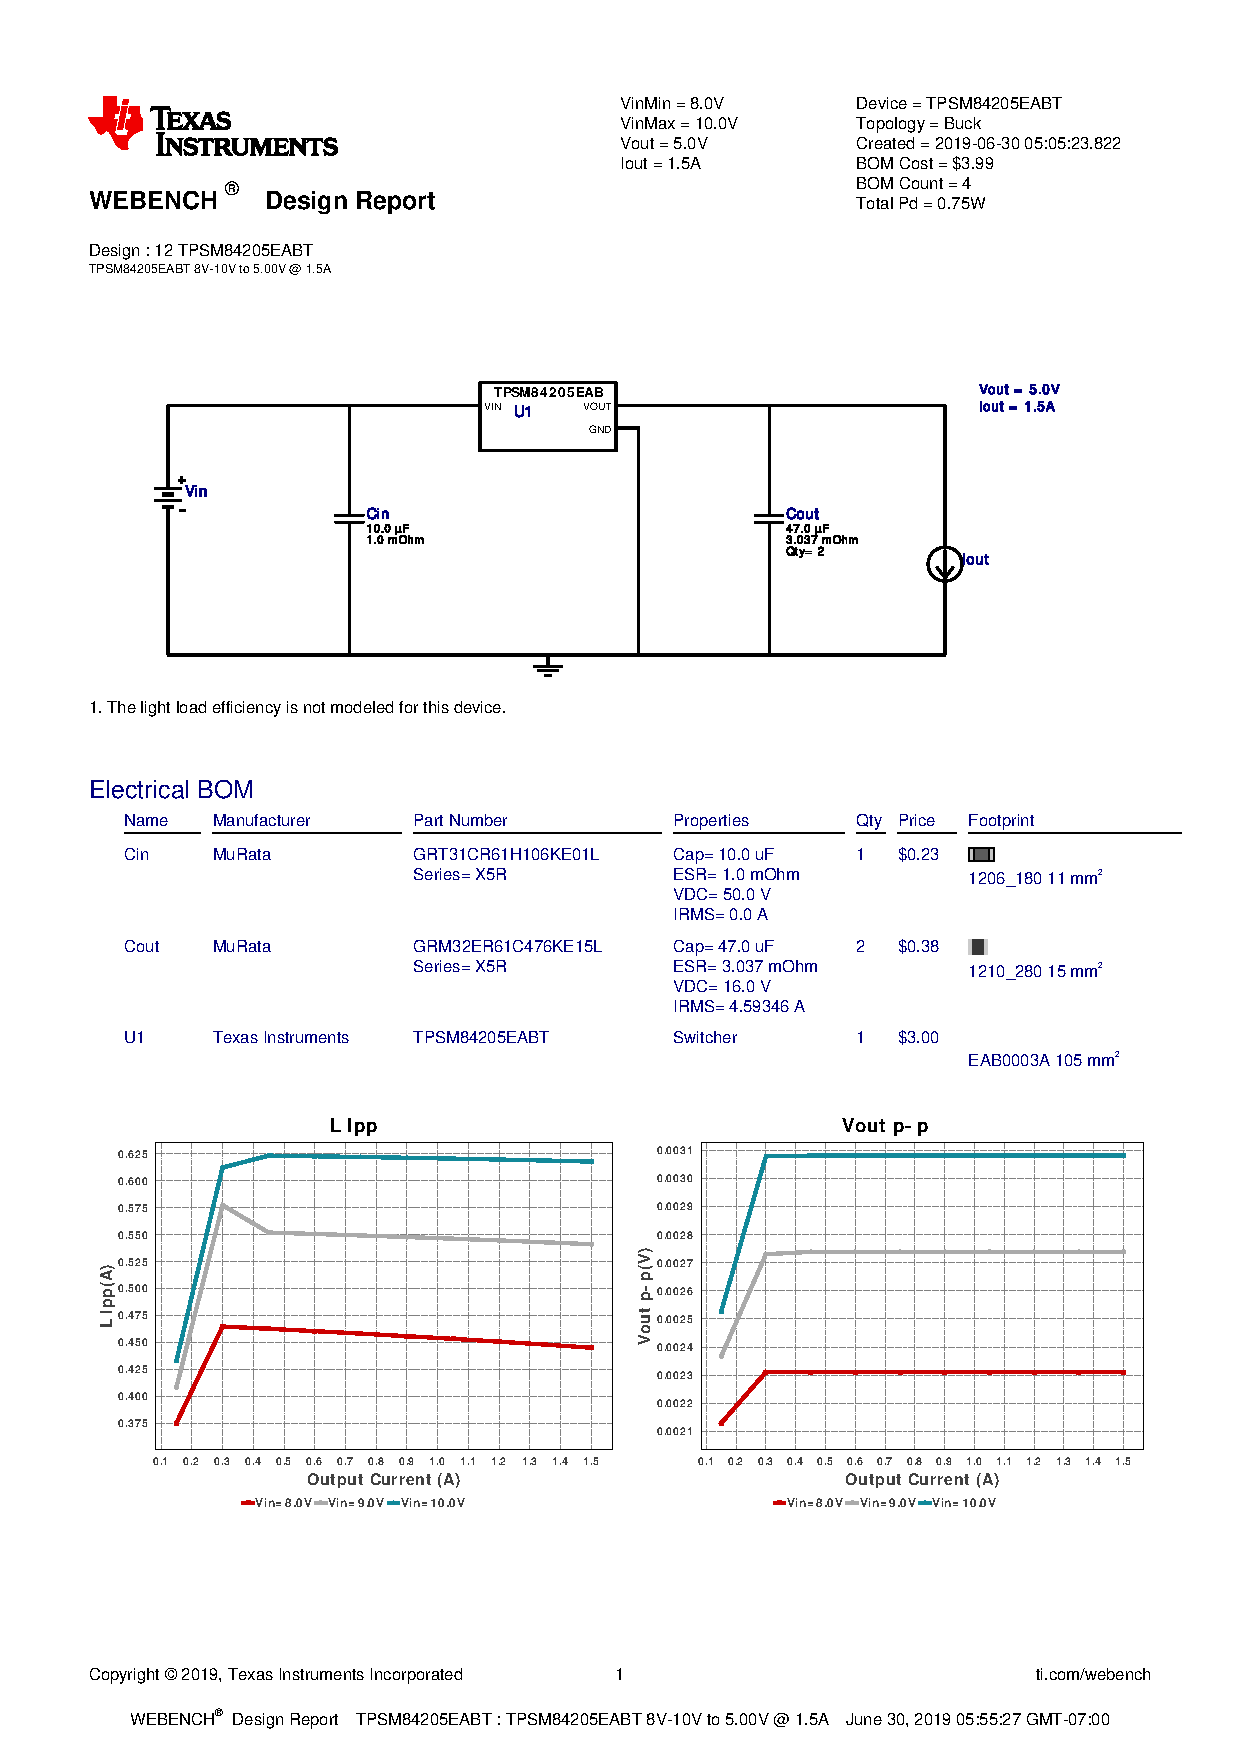
\includegraphics[width = 0.98\textwidth]{wb_report_cover.pdf}
\end{figure}

% \newpage
% \section{常用格式待查}

% \subsection{文本编辑}
% \paragraph{}
% \textbf{加粗}\footnote{脚注}\textit{斜体}
% \vspace{1cm}%水平间距调整
% \vskip 7cm %垂直间距调整


% \textbf{加粗}
% \footnote{footnote}
% \par{} 强制段落和缩进测试,人类的本质是复读机,人类的本质是复读机,人类的本质是复读机,人类的本质是复读机
% \par{} 强制段落和缩进测试par用来缩进,人类的本质是复读机,人类的本质是复读机,人类的本质是复读机,人类的本质是复读机\S chapter
% \paragraph{paragraph用来加这个粗字} 强制段落和缩进测试pargraph没有,人类的本质是复读机,人类的本质是复读机,人类的本质是复读机,人类的本质是复读机

% \subsection{图}

% \begin{figure}[H]
%     \centering
%     \includegraphics[width = 0.8\textwidth]{test.png}
%     \caption{标题} %最终文档中希望显示的图片标题
%     \label{test}
% \end{figure}

% \par{} 引用测试 图\ref{test}

% \begin{figure}[H]
%   \centering
%   \begin{minipage}[H]{0.48\textwidth}
%     \centering
%     \includegraphics[width = 0.9\textwidth]{test.png}
%     \caption{标题1}
%   \end{minipage}
%   \begin{minipage}[H]{0.48\textwidth}
%     \centering
%     \includegraphics[width = 0.9\textwidth]{test.png}
%     \caption{标题2}
%   \end{minipage}
% \end{figure}

% 正常的段落

% \begin{wrapfigure}{r}{0pt}    
%     \includegraphics[width = 0.4\textwidth]{test.png}
%     \caption{right hand side}
% \end{wrapfigure}

% 我就正常写个段落,他会在左边。我就正常写个段落,他会在左边。我就正常写个段落,他会在左边。我就正常写个段落,他会在左边。我就正常写个段落,他会在左边。我就正常写个段落,他会在左边。我就正常写个段落,他会在左边。我就正常写个段落,他会在左边。我就正常写个段落,他会在左边。我就正常写个段落,他会在左边。我就正常写个段落,他会在左边。我就正常写个段落,他会在左边。我就正常写个段落,他会在左边。我就正常写个段落,他会在左边。我就正常写个段落,他会在左边。我就正常写个段落,他会在左边。我就正常写个段落,他会在左边。我就正常写个段落,他会在左边。我就正常写个段落,他会在左边。我就正常写个段落,他会在左边。

% \newpage
% \subsection{数学}
% \par{} 引用测试 \ref{test}

% \paragraph{} the theorem is named after Russian Al. In this variant of the \textbf{CLT} the random $X_i + \sigma$

% \paragraph{} Suppose ${X_1,X_2,...}$ is a sequence of independent random variables, each with finite expected value $\mu_i$ and variance $\sigma^2$. Define
% \begin{equation}
%    s_n^2=\sum_{i=1}^n \sigma_i^2 \qquad i = 1,2, \cdots n
% \end{equation}

% \begin{equation*}
%   \int_{a}^{b}f(x) \,\mathrm{d}x = \frac{\mathrm{d}p}{\mathrm{d}q}
% \end{equation*}

% \begin{align*}
%     P(X(S_n)=k-1|X(S_{n-1})=k)&=1\\
%     P(X(S_n)=i,i\neq k-1|X(S_{n-1})=k)&=0
% \end{align*}

% \begin{equation}
%     P=\left[ \begin{array}{ccccc}
%          0&0&\cdots&0&1  \\
%          1&0&\cdots&0&0 \\
%          0&1&\cdots&0&0\\
%          \vdots&\vdots&\ddots&\vdots&\vdots\\
%          0&0&\cdots&1&0
%     \end{array} \right]
% \end{equation}

% % physics package to get a more readable formulation but cannot get the hold preview

% \begin{equation*}
%   \dv{f}{x} = \pdv[n]{g}{t} = \pdv{f}{x}{y} = \mqty(a & b \\ c & d) = \int_{a}^{b}\sin[2](x) \dd x  = \abs{a} \qq{quick insert word}
% \end{equation*}

% \subsection{表}
% % use latex table tool-- an online generator tool to fast build a table
%   \begin{table}[H]
%     \centering
%       \begin{tabular}{cc}
%           A & a\\
%           BBB & b\\
%       \end{tabular}
%     \caption{test}
%   \end{table}

%   \begin{table}[H]
%     \centering
%     \begin{tabular}{||c|c|c|c||}
%       \hline
%       \multirow{2}*{合并行}&\multicolumn{3}{c||}{合并列}\\
%       \cline{2-4}
%       &测试&测试&测试\\
%       \hline
%       \end{tabular}
%     \caption{muti table}
%   \end{table}

%   \begin{table}[H]
%     \centering
%     \begin{threeparttable}
%       \small 
%       \begin{tabular} {llll}
%         \toprule
%         GDP in base year(2010)/billion\$ & $A/A'$ & $S/S'$ & $G/G'$ \\
%         \midrule
%         123.166  & 2.187 & 1.129 & 1.471 \\
%         \bottomrule
%       \end{tabular}
%       \caption{Vietnam economic indicators}
%     \end{threeparttable}
%   \end{table}



% \subsection{代码}

% \begin{lstlisting}[caption = c++ hellow world]
% #include<iostream>
% int main() {
%     int a;
%     for (int i = 0; i < 100; i++) {
%       if (i % 2 == 0) {
%         printf("Hello World!");
%       }
%     }
%   return 0;
% }
% \end{lstlisting}

% % use [language to change the para in lstset] to 
% \begin{lstlisting}[language = python, caption = py hellow world]
% for c in 'Python'
%     print(c + '!')
% \end{lstlisting}

% \subsection{条目列表}

% \begin{itemize}
%   \item[*]INIT$\to$START: 按下START
%   \item[*]INIT$\to$INIT: 未按下START 
%   \item[*]START$\to$INPUT: START状态用于将输出的money, timer置为0,故此次态必为INPUT
%   \item[*]INPUT$\to$INPUT: 没有按下ok,继续输入数字
% \end{itemize}

% \subsection{制图}
% % may be warning incomptiable color with lstlisting ,recommand compile figure alone and insert to avoid it and speed up document compile
% \begin{figure}[H]
% \centering 
% \begin{tikzpicture}[scale = 0.8] % or width with textwidth
%   \draw[help lines] (8, 8) grid(11,11);
%   \draw [->] (8, 8) --(9, 11);
%   \draw [<->][line width = 2][black][dashed] (8,10) -- (8,8) -- (11,8);
%   \draw[blue] (11,12) rectangle(10, 11);
%   \draw[blue, fill = orange] (10,13) circle[radius = 0.1];
%   \node[below] at (10, 13) {label $m \alpha th$};
%   \draw [thick, black] (8,8) to [out=90,in=180] (9,9) to [out=0,in=180] (10.5,8) to [out=0,in=-135] (12,9) node[right, black]{in out degree curve};
%   \node at (12,13) {free label $m \alpha th$};
  
%   \path [fill=yellow] (0,0) -- (0,5) to [out=-80, in=160] (3,.8) -- (3,0) -- (0,0);
%   \draw [<->] (0,6) node [left] {$P$} -- (0,0) node [below left] {(0,0)} -- (7,0) node [below] {$Q$};
%   \draw [ultra thick, dashed] (0,.8) node [left] {$P^*=.8$} -- (3,.8) -- (3,0) node [below] {$Q^*=3$};
%   \draw [fill] (3,.8) circle [radius=.1];
%   \draw [thick] (0,5) to [out=-80, in=160] (3,.8) to [out=-20, in=175] (6,0);     
%   \end{tikzpicture}
%   \caption{tikz制图供求曲线以及右上角的杂图}
% \end{figure}

% \begin{tikzpicture}
%   \draw
%   (0, 2) node[and port] (myand1) {}
%   (0, 0) node[and port] (myand2) {}
%   (2, 1) node[xnor port] (myxnor) {}
%   (myand1.out) -| (myxnor.in 1)
%   (myand2.out) -| (myxnor.in 2);
% \end{tikzpicture}

% \begin{figure}[H]
%     \centering
%     \begin{tikzpicture}
%       \draw
%       (4, 0) node[rground] (ground){}
%       (4, 3) node[npn] (npn) {}
%       (4, 6) node[rground, rotate = 180] (vcc) {} (4, 6) node[right] {$V_{cc}$}
%       (0, 3) to[C, l_=$C_1$,  v^<=$U_{BEQ}$] (2, 3)
%       (0, 3) node[] (C1n) {} (2, 3) node[] (C1p) {}
%       (4, 4) to[C, l_=$C_2$,  v^>=$U_{CEQ}$] (6, 4)
%       (4, 4) node[] (C2p) {} (6, 4) node[] (C2n) {}
%       (3, 5) to[R, l=$R_b$] (3, 3)
%       (3, 5) node[] (Rbp) {} (3, 3) node[] (Rbn) {}
%       (4, 4) to[R, l=$R_c$] (4, 6)
%       (4, 4) node[] (Rcn) {}  (4, 6) node[] (Rcp) {}
%       (6, 1) to[R, l=$R_L$] (6, 3)
%       (6, 1) node[] (RLn) {}  (6, 3) node[] (RLp) {}
%       ;
%       \draw
%       (C1n) to[short, o-] (C1n)
%       (C2n) to[short, o-] (C2n)
%       (Rbn) to[short, *-] (npn.B)
%       (C1p) to[short, -*] (Rbn)
%       (Rbp) to[short] (3, 6) to[short, -*] (vcc)
%       (Rcp) to[short, -*] (vcc)
%       (npn.C) to[short, -*] (Rcn)
%       (0, 0) to[short, o-*] (ground) to[short, *-o] (6, 0)
%       (ground) to[short, *-] (npn.E)
%       ;
%       \draw[dashed]
%       (6, 0) to[short] (RLn)
%       (C2n) to[short] (RLp)
%       ;
%       \draw
%       (C1n) node[below] {$+$} (0, 0) node[above] {$-$}
%       (C2n) node[right] {$+$} (6, 0) node[right] {$-$}
%       (0, 1.5) node[] {$u_i$}
%       (6.2, 2) node[right] {$u_o$}
%       ;
% \end{tikzpicture}
%     \caption{amplifer circuit(by circuitikz)}
% \end{figure}

% \newpage
% \appendix % into appendix mode, section will count as ABCD

% \section{图表源码索引}

% \listoffigures
% \listoftables
% \lstlistoflistings % code listing

\end{document}
